\subsection{Topological comparison of neural dynamics on the entropy--cost plane}

We now ask whether the three systems characterized above (single-neuron model, recurrent network, V1 data) share the geometric organization predicted by the Gibbs manifold when projected onto a common entropy--cost plane.  For each system we plot information rate $I$ (or entropy rate $H$ in the spontaneous case) against metabolic cost $C$, and ICE $=I/C$ against $C$, in common absolute units (bits/s and W).  The Gibbs manifold in every panel is
\begin{equation}
H(C) \approx I(C) = \frac{R_0}{\ln 2}\left[1 + \ln\!\left(\frac{C-2.4}{0.37}\right)\right] \; [\text{bits/s}].
\label{eq:entropy_rate}
\end{equation}
Equation~\eqref{eq:entropy_rate} is the linear-cost asymptote: under $C(r)=C_0+C_1 r$ with $C_0=2.4$\,W, $C_1=0.37$\,W/Hz \cite{Yuguo2018Evaluating}, the unbounded-linear-cost Gibbs solution is exponential with mean $(C-C_0)/C_1$ and entropy $1+\ln\langle r\rangle$ nats; converting to bits and rescaling by $R_0$ gives the displayed rate (bounded-domain and sublinear forms in Supp.~Sect.~1.4, 1.7).

\paragraph{Per-system rate calibration.}
Converting per-observation entropy to an information rate requires one scale factor $R_0$ per system (the rate of independent observations used to form spike words).  $R_0$ is not fitted to the manifold but fixed by anchoring a single empirical point on the manifold.  For the two model systems the trajectory is tight and the minimum-rate point provides a clean upper-envelope anchor ($R_0=1.63$ for the single neuron, $R_0=1.0$ for the recurrent network).  For V1, where the empirical scatter spans the full cost axis, the minimum-rate point is poorly determined; we therefore anchor at the median rate ($R_0=2.58$), which renders the manifold as a representative central trend through the data cloud rather than a strict upper bound.  Anchor sensitivity for V1 is characterized in Supp.~Fig.~S7: the trajectory topology and the $\mathrm{ICE}>\beta$ inequality are anchor-invariant; only the absolute scale and data-to-manifold gap depend on the anchor.

\paragraph{Manifold-like organization across systems.}
All three systems trace concave trajectories whose shape is consistent with the Gibbs manifold (Fig.~\ref{fig:Gibbs-frontier}, top row), a topological alignment after system-specific rate calibration rather than a parameter-free collapse.  The two model systems (A, B) migrate from low-$C$, low-$I$ initial states toward the manifold (grey arrows), while V1 (C) lies below the manifold across the full cost range; this asymmetry reflects a difference in measurement, not in shape.  The model panels show \emph{learning trajectories} (proximity to the manifold is the asymptote of plasticity); the V1 panel shows \emph{instantaneous operating points} aggregated across cells and trials, with the vertical gap to the manifold set by the empirical noise-entropy fraction $\bar\rho\approx 0.85$ (Section~\ref{sec:cv_s_data}).  Spontaneous V1 activity ($H$) reaches higher information rates than evoked ($I$) at matched cost, reflecting the gap between available coding capacity and deployed capacity.

\paragraph{Concavity inequality.}
Replotted as the average-efficiency curve $\mathrm{ICE}=I/C$ vs.\ $C$ (Fig.~\ref{fig:Gibbs-frontier}, bottom row), the data exhibit the concavity inequality $\mathrm{ICE}>\beta$ within each system, where $\beta=dI/dC$ is the marginal efficiency: because $I^{\star}(C)$ is strictly concave, the secant $I/C$ always exceeds the local slope $dI/dC$.  In V1 the spontaneous cluster (inset) occupies the steep low-cost corner where ICE is maximized, consistent with the resting state maintaining maximal coding capacity within a tight metabolic budget~\cite{Raichle2001}.

\begin{figure}[!h]
\centering
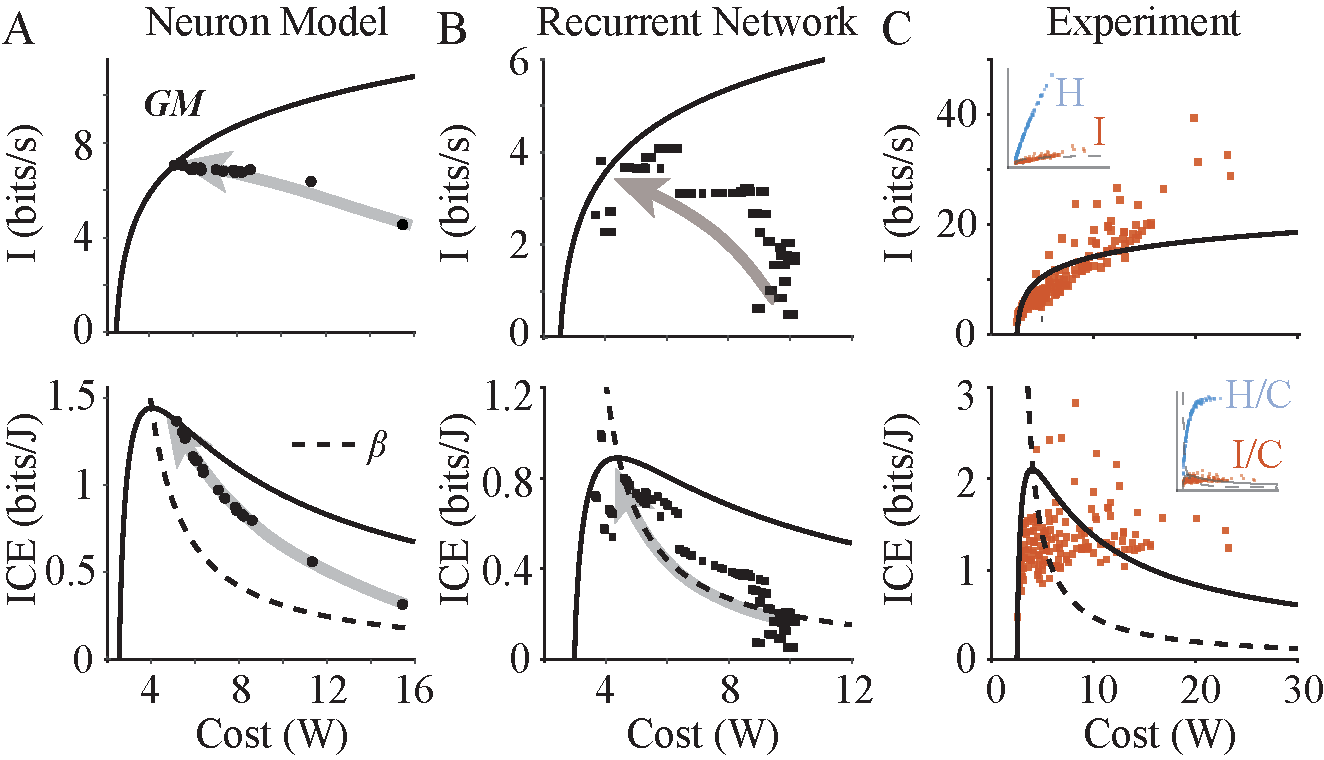
\includegraphics[scale=0.4]{figures/Figure5.pdf}
\caption{\textbf{Trajectories align with the Gibbs manifold on the entropy--cost plane after system-specific rate calibration.}  Columns: (\textbf{A})~single-neuron LIF model, (\textbf{B})~recurrent spiking network, (\textbf{C})~macaque V1.  \textbf{Top}: information rate vs.\ cost; $I$ for evoked (black in A--B, orange in C), $H$ for V1 spontaneous (blue; entropy/coding-readiness units, not stimulus information).  Dashed: Gibbs manifold $H^\star(C)$ (Eq.~\ref{eq:entropy_rate}) with per-system $R_0$ anchors $1.63/1.0/2.58$ for A/B/C.  A/B use the minimum-rate anchor (manifold = upper envelope; the model trajectory is short and tight, so the lowest-rate point is well-determined); C uses the median-rate anchor (manifold = central trend through the V1 cloud, since the minimum-rate point is dominated by a single low-FR outlier).  Topology (concavity, $\mathrm{ICE}>\beta$, rank ordering) is anchor-invariant; only the absolute scale and data-to-manifold gap depend on the anchor (Supp.~Fig.~S7).  \textbf{Bottom}: average-efficiency curve $\mathrm{ICE}(C)=H^\star/C$ (solid black) and marginal-efficiency curve $\beta(C)=dI/dC$ (dashed).  The concavity inequality $\mathrm{ICE}>\beta$ holds within each system.  Panel C bottom: evoked $I/C$ in main axes for cross-column comparability; spontaneous $H/C$ in inset (high-ICE, low-cost corner).  Grey arrows in A, B: learning direction; in C each dot is an instantaneous operating point.  Cross-column absolute units are not directly comparable.}
\label{fig:Gibbs-frontier}
\end{figure}
